\chapter{Signal Fits}


\begin{figure}
	\begin{center}
		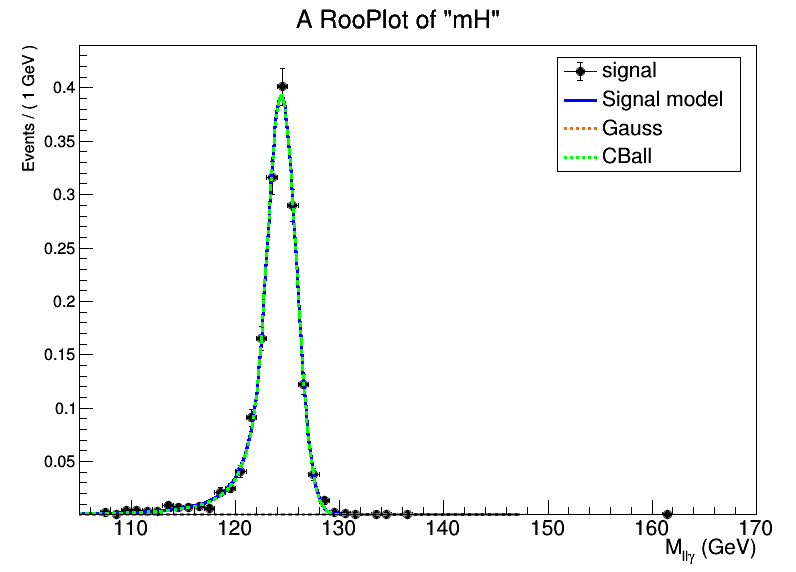
\includegraphics[width=0.40\textwidth]{fig/signal_fit/2017/sigfit_ele_ggF_1_125.png}
		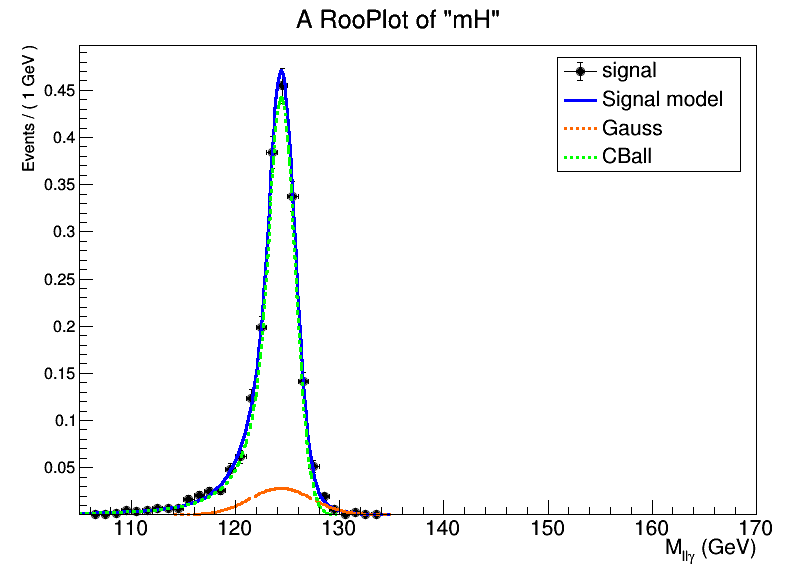
\includegraphics[width=0.40\textwidth]{fig/signal_fit/2017/sigfit_ele_ggF_2_125.png}\\
		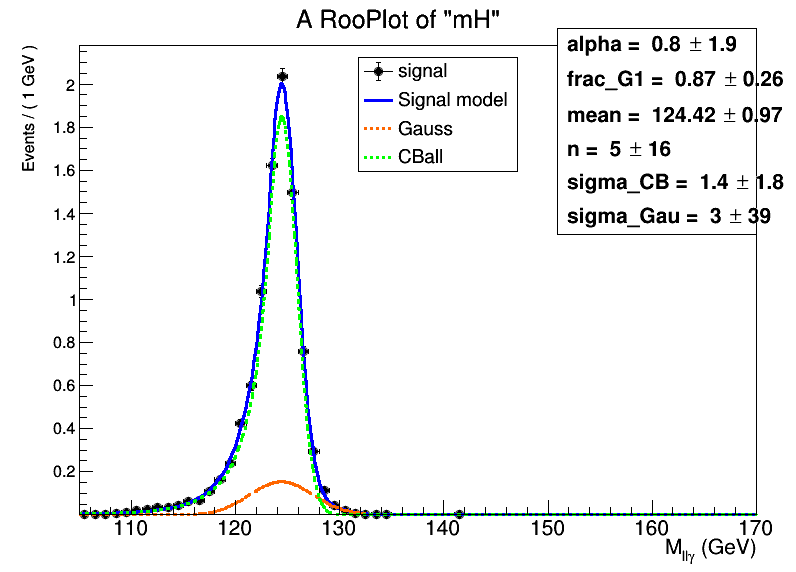
\includegraphics[width=0.40\textwidth]{fig/signal_fit/2017/sigfit_ele_ggF_3_125.png}
		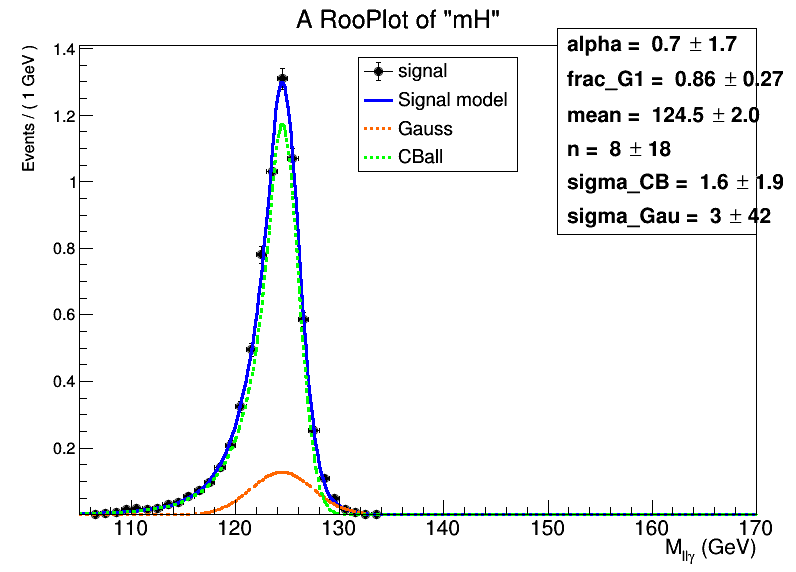
\includegraphics[width=0.40\textwidth]{fig/signal_fit/2017/sigfit_ele_ggF_4_125.png}\\
		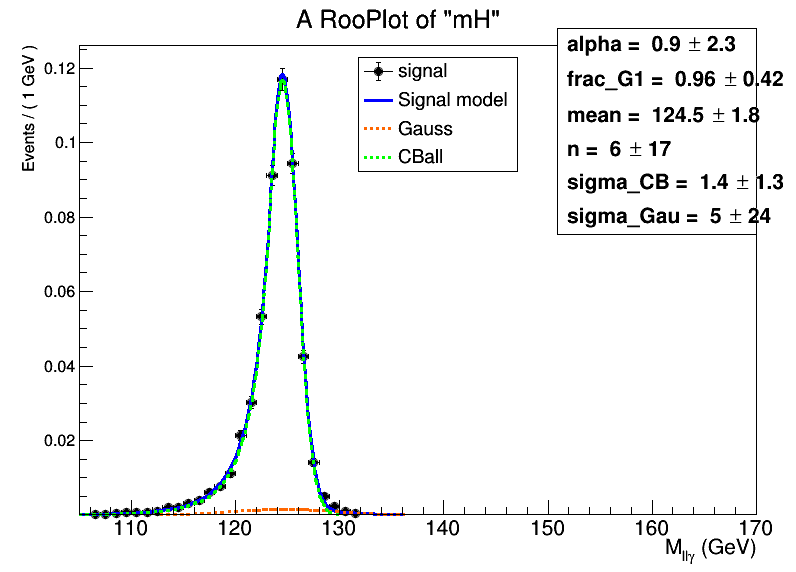
\includegraphics[width=0.40\textwidth]{fig/signal_fit/2017/sigfit_ele_VBF_501_125.png}
		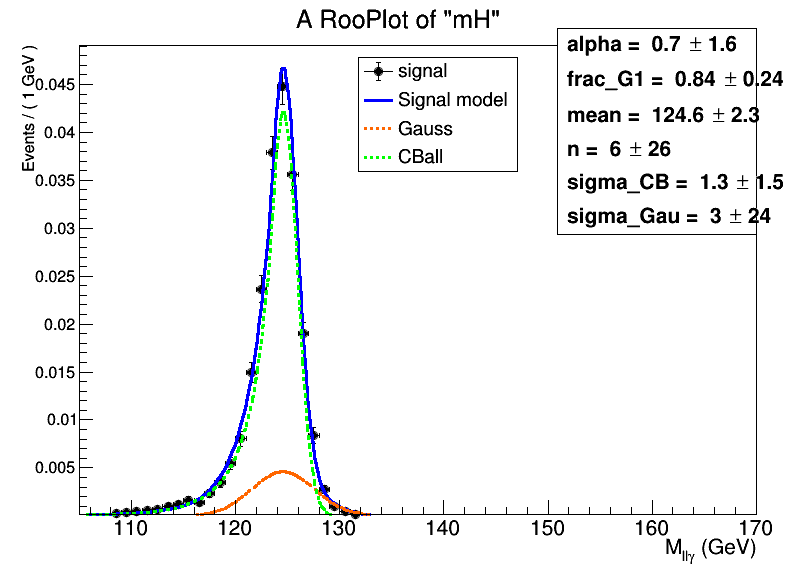
\includegraphics[width=0.40\textwidth]{fig/signal_fit/2017/sigfit_ele_VBF_502_125.png}\\
		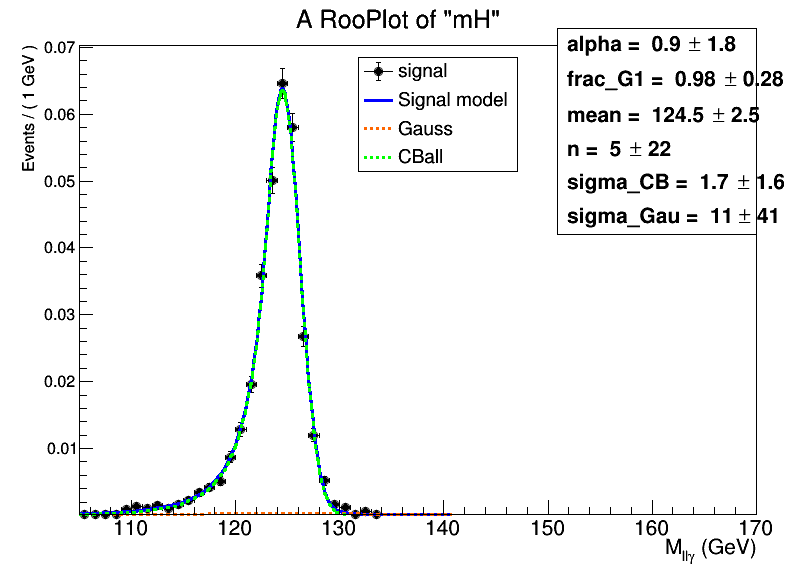
\includegraphics[width=0.40\textwidth]{fig/signal_fit/2017/sigfit_ele_VBF_503_125.png}\\
		\caption{Fits to simulated $m_{\ell^+\ell^-\gamma}$ signal distributions in the electron channel for
            		 $m_\PH=125\GeV$ for the 2017 data-taking period.
			 The blue line shows the total fit function, the green line shows the Crystal Ball function component, and the red line shows the Gaussian function component.
			 The top four plots correspond to the untagged categories, and the bottom three plots correspond to the dijet categories.}
		\label{fig:elesigfit}
	\end{center}
\end{figure}

\begin{figure}
	\begin{center}
		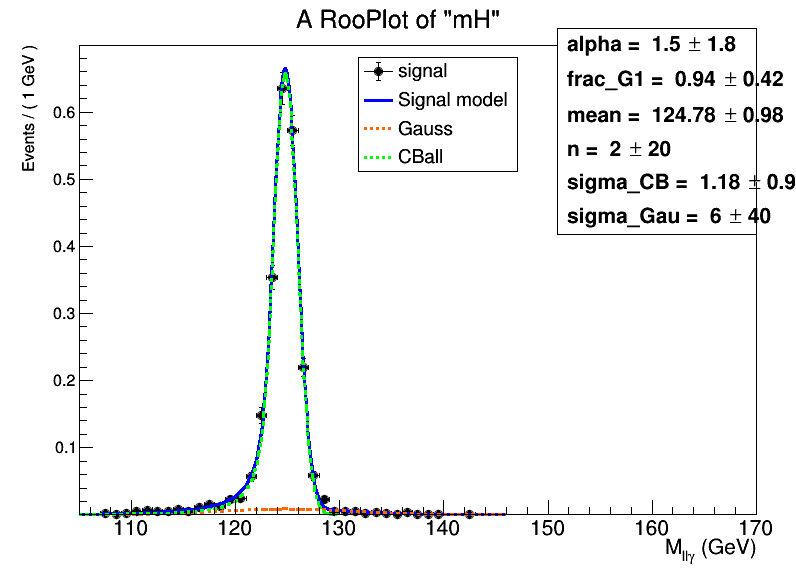
\includegraphics[width=0.40\textwidth]{fig/signal_fit/2017/sigfit_mu_ggF_1_125.png}
		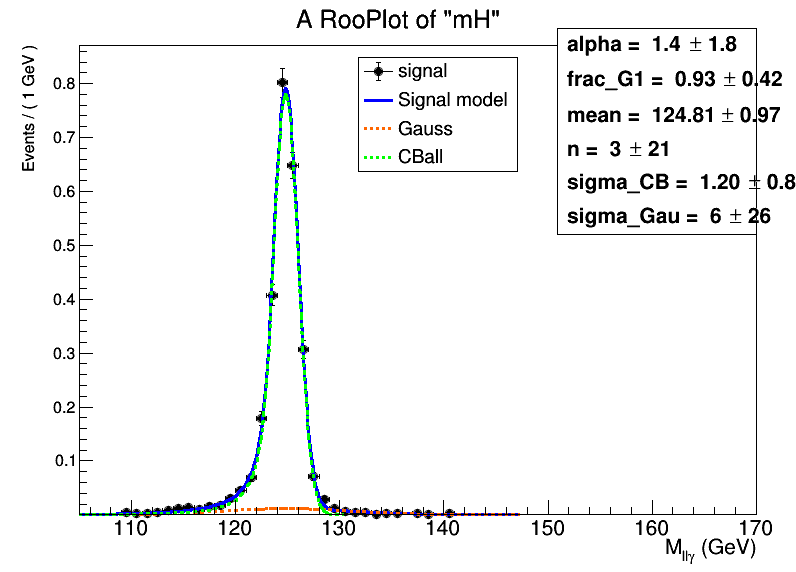
\includegraphics[width=0.40\textwidth]{fig/signal_fit/2017/sigfit_mu_ggF_2_125.png}\\
		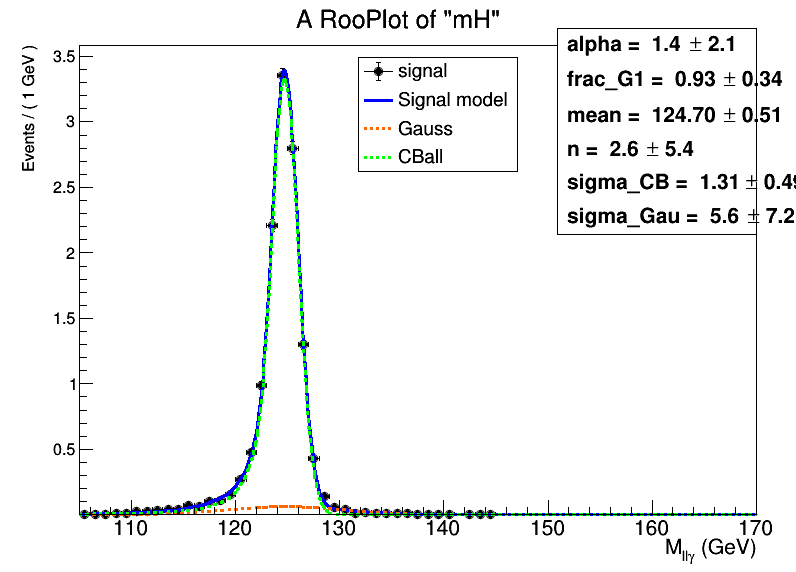
\includegraphics[width=0.40\textwidth]{fig/signal_fit/2017/sigfit_mu_ggF_3_125.png}
		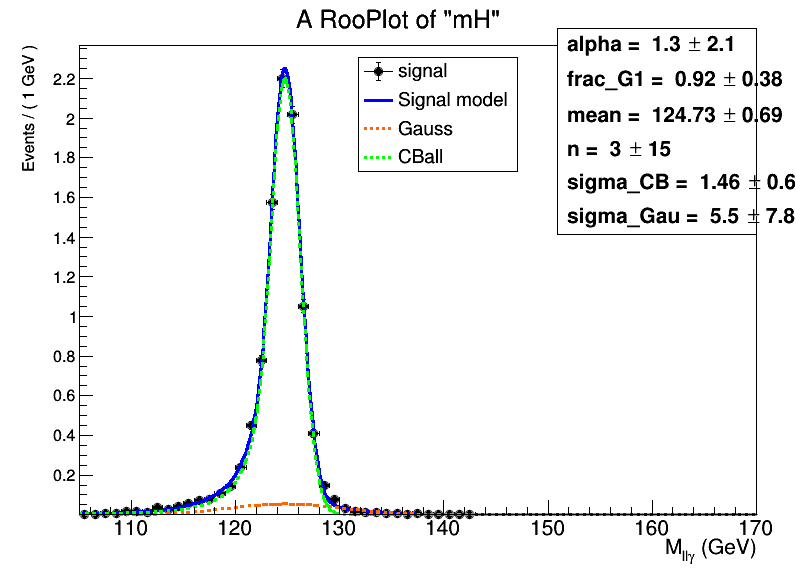
\includegraphics[width=0.40\textwidth]{fig/signal_fit/2017/sigfit_mu_ggF_4_125.png}\\
		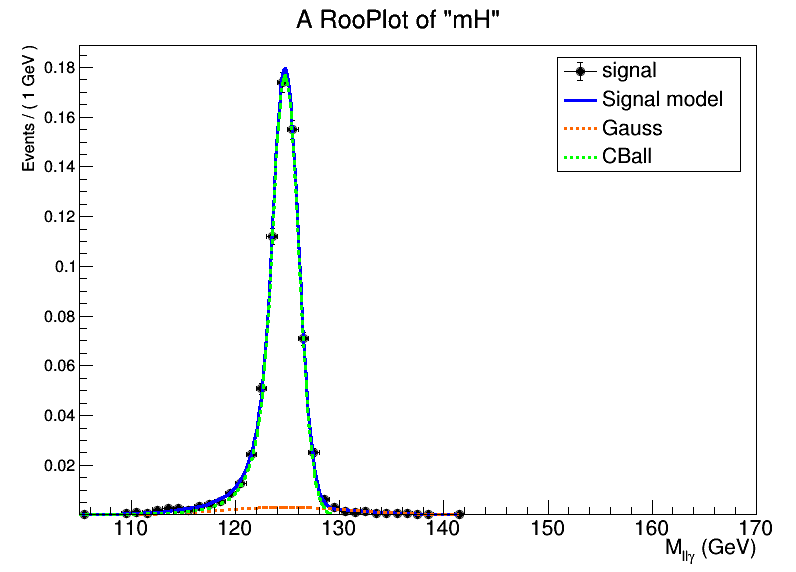
\includegraphics[width=0.40\textwidth]{fig/signal_fit/2017/sigfit_mu_VBF_501_125.png}
		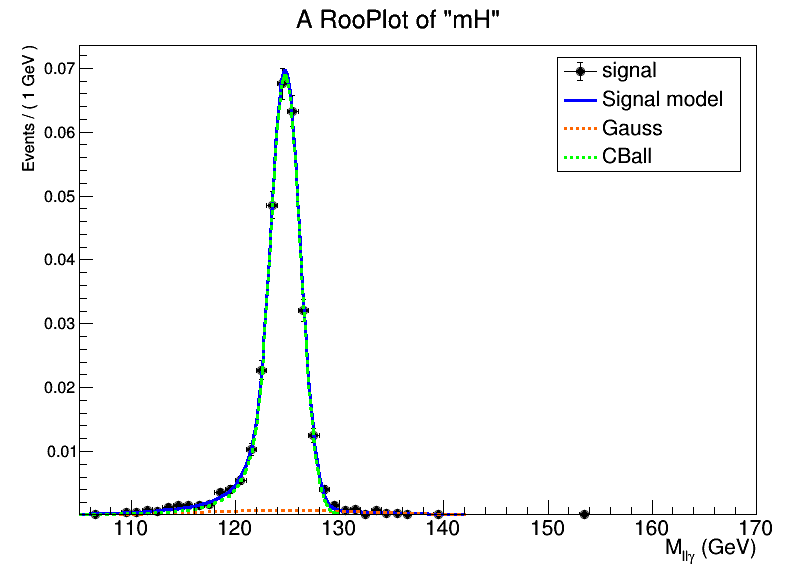
\includegraphics[width=0.40\textwidth]{fig/signal_fit/2017/sigfit_mu_VBF_502_125.png}\\
		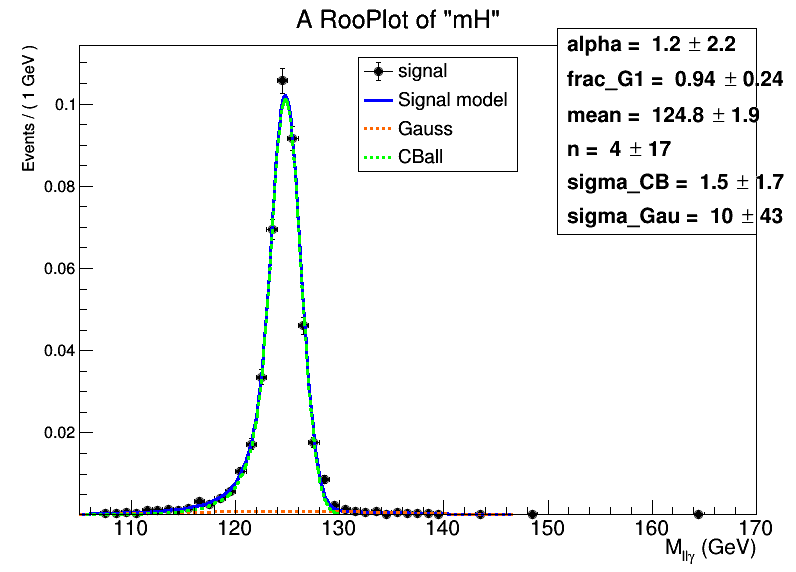
\includegraphics[width=0.40\textwidth]{fig/signal_fit/2017/sigfit_mu_VBF_503_125.png}\\
		\caption{Fits to simulated $m_{\ell^+\ell^-\gamma}$ signal distributions in the muon channel for
            		 $m_\PH=125\GeV$ for the 2017 data-taking period.
			 The blue line shows the total fit function, the green line shows the Crystal Ball function component, and the red line shows the Gaussian function component.
			 The top four plots correspond to the untagged categories, and the bottom three plots correspond to the dijet categories.}
		\label{fig:elesigfit}
	\end{center}
\end{figure}

\begin{figure}
	\begin{center}
	  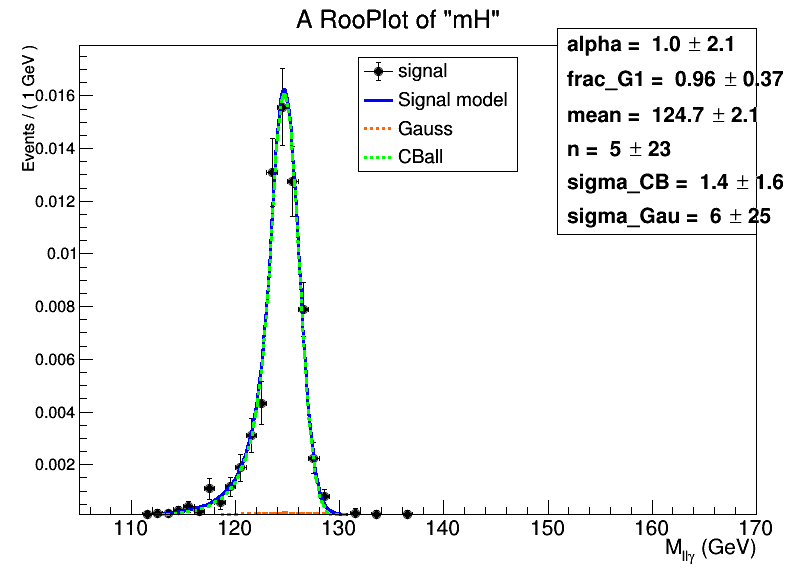
\includegraphics[width=0.40\textwidth]{fig/signal_fit/2017/sigfit_ele_mu_ZH_6789_125.png}
	  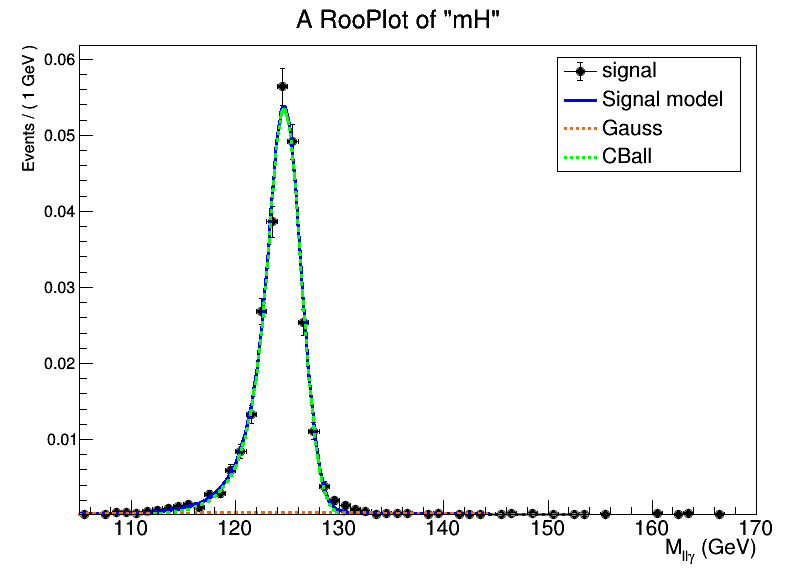
\includegraphics[width=0.40\textwidth]{fig/signal_fit/2017/sigfit_ele_mu_WH_6789_125.png}
		\caption{Fits to simulated $m_{\ell^+\ell^-\gamma}$ signal distributions in the electron and muon channels combined in the lepton-tagged category for
            		 $m_\PH=125\GeV$ for the 2017 data-taking period.
        		 The left plot shows the fit to simulated ZH production events, and the right plot shows the fit to simulated WH production events. 
			 The blue line shows the total fit function, the green line shows the Crystal Ball function component, and the red line shows the Gaussian function component.}
		\label{fig:elemusigfit}
	\end{center}
\end{figure}

\begin{figure}
	\begin{center}
		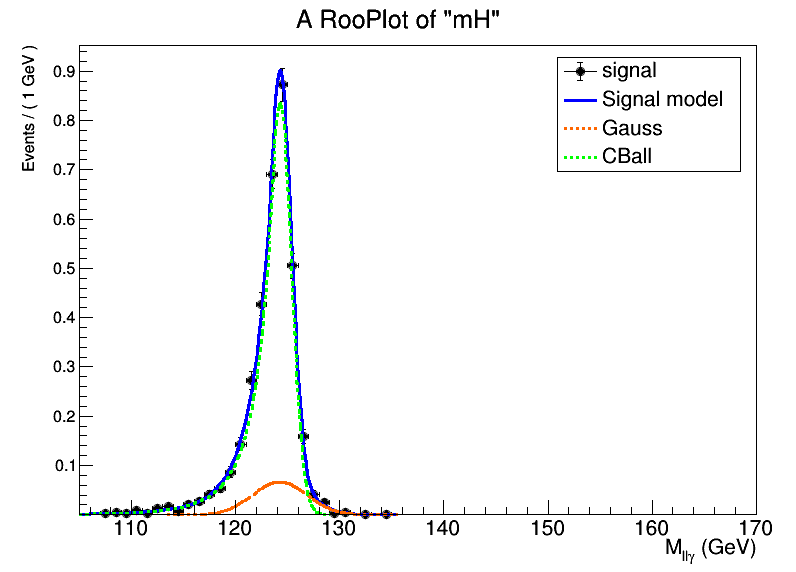
\includegraphics[width=0.40\textwidth]{fig/signal_fit/2018/sigfit_ele_ggF_1_125.png}
		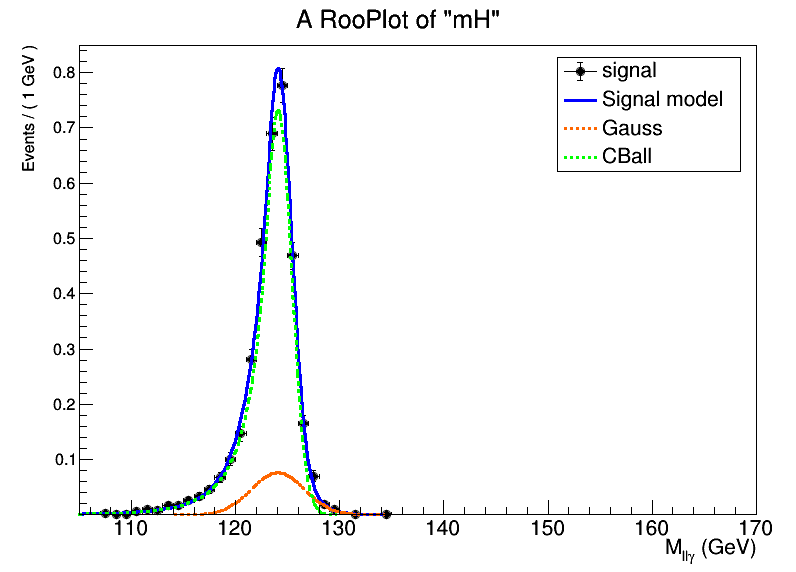
\includegraphics[width=0.40\textwidth]{fig/signal_fit/2018/sigfit_ele_ggF_2_125.png}\\
		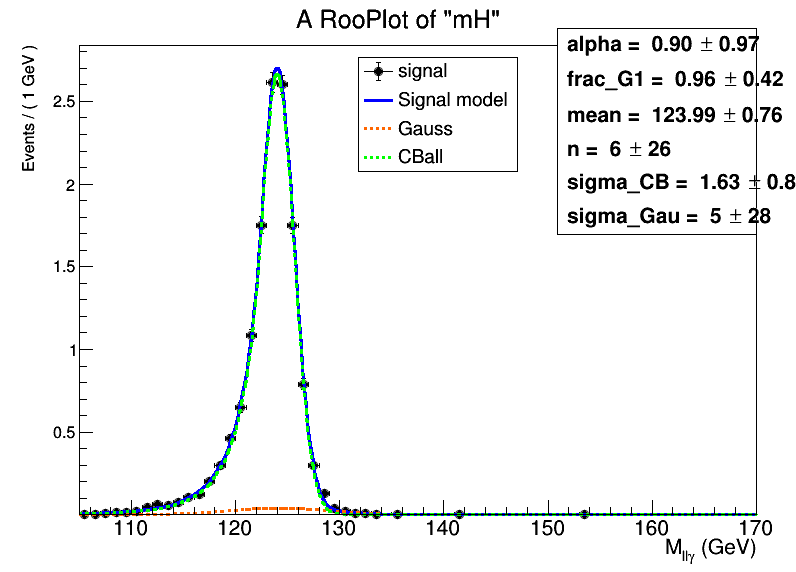
\includegraphics[width=0.40\textwidth]{fig/signal_fit/2018/sigfit_ele_ggF_3_125.png}
		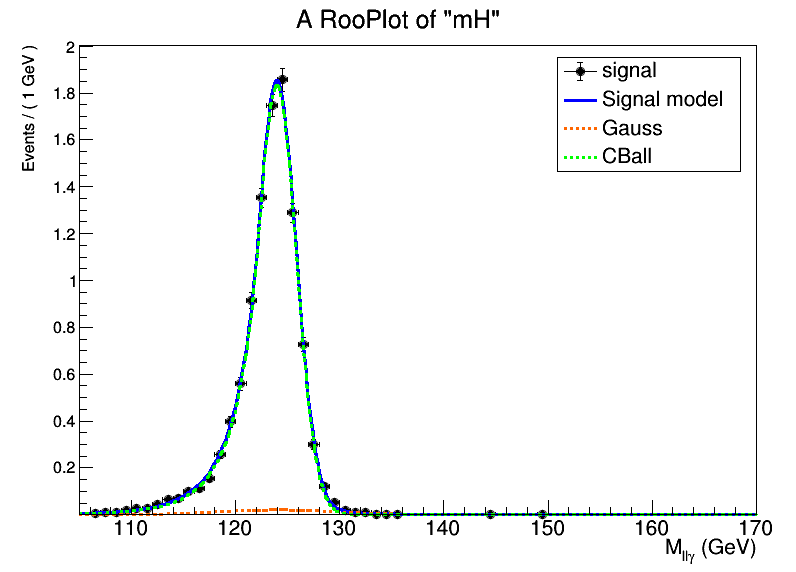
\includegraphics[width=0.40\textwidth]{fig/signal_fit/2018/sigfit_ele_ggF_4_125.png}\\
		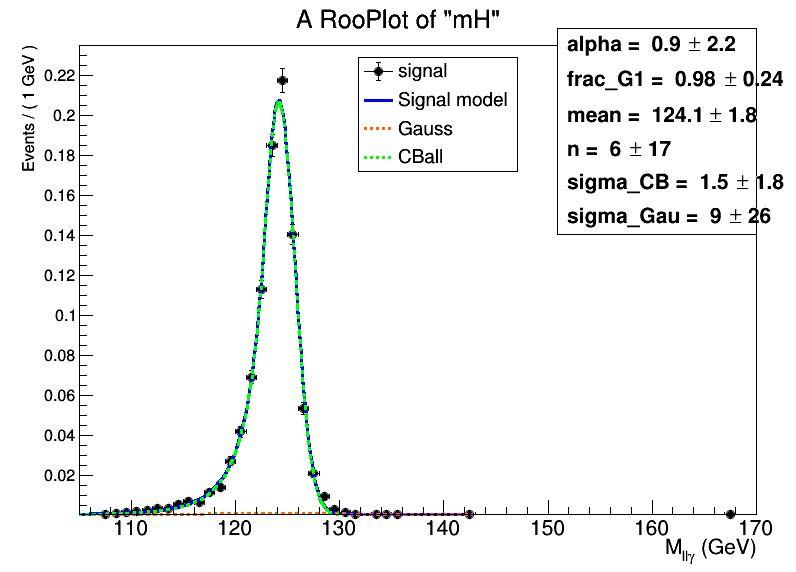
\includegraphics[width=0.40\textwidth]{fig/signal_fit/2018/sigfit_ele_VBF_501_125.png}
		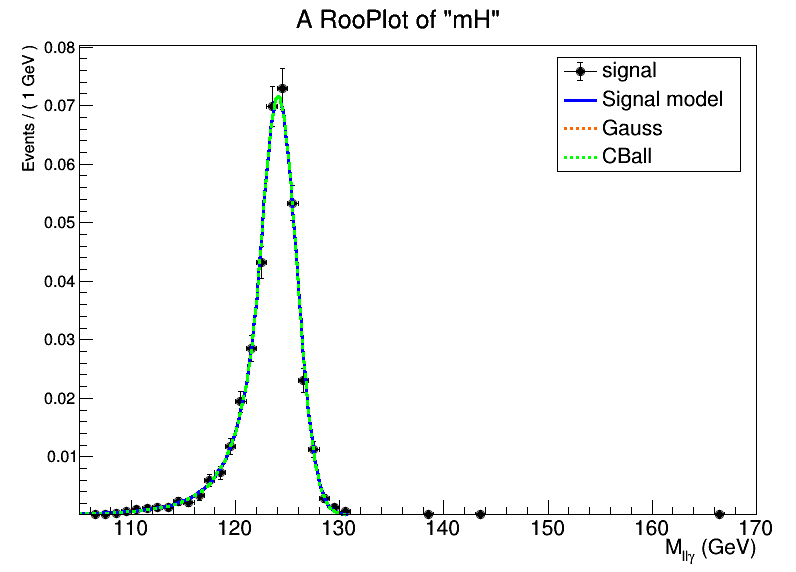
\includegraphics[width=0.40\textwidth]{fig/signal_fit/2018/sigfit_ele_VBF_502_125.png}\\
		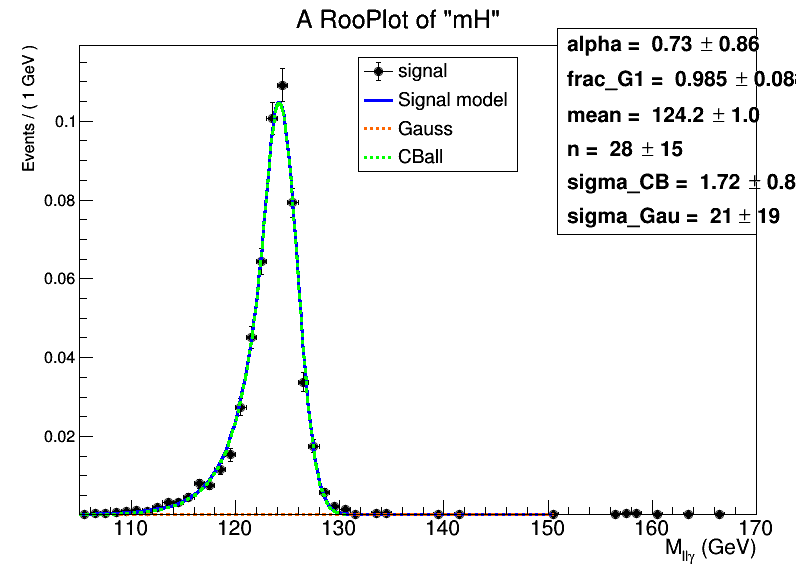
\includegraphics[width=0.40\textwidth]{fig/signal_fit/2018/sigfit_ele_VBF_503_125.png}\\
		\caption{Fits to simulated $m_{\ell^+\ell^-\gamma}$ signal distributions in the electron channel for
            		 $m_\PH=125\GeV$ for the 2018 data-taking period.
			 The blue line shows the total fit function, the green line shows the Crystal Ball function component, and the red line shows the Gaussian function component.
			 The top four plots correspond to the untagged categories, and the bottom three plots correspond to the dijet categories.}
		\label{fig:elesigfit}
	\end{center}
\end{figure}

\begin{figure}
	\begin{center}
		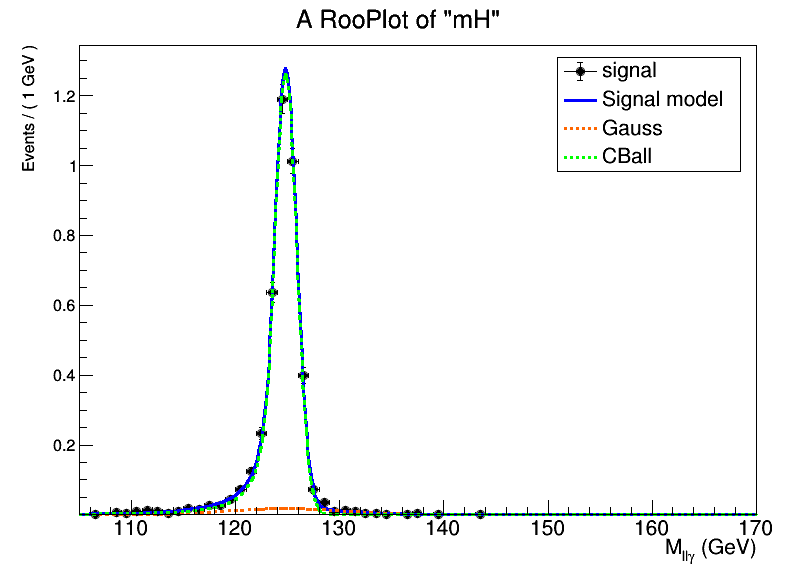
\includegraphics[width=0.40\textwidth]{fig/signal_fit/2018/sigfit_mu_ggF_1_125.png}
		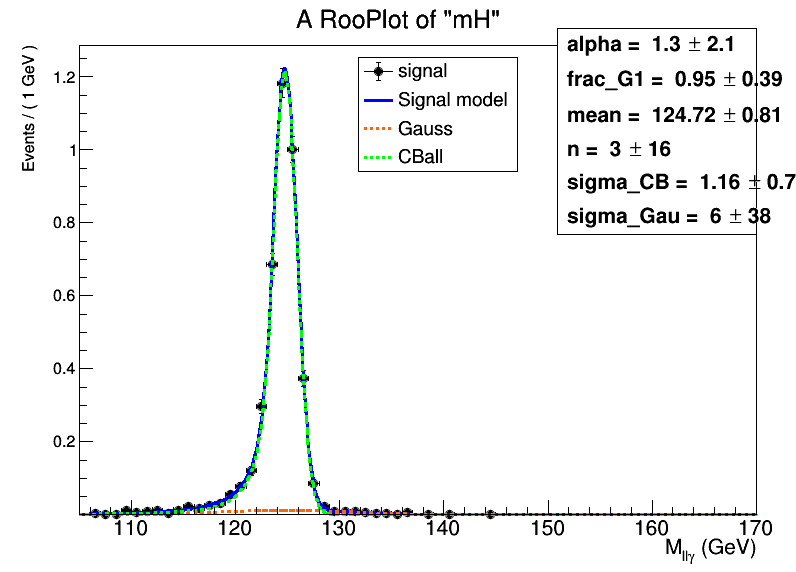
\includegraphics[width=0.40\textwidth]{fig/signal_fit/2018/sigfit_mu_ggF_2_125.png}\\
		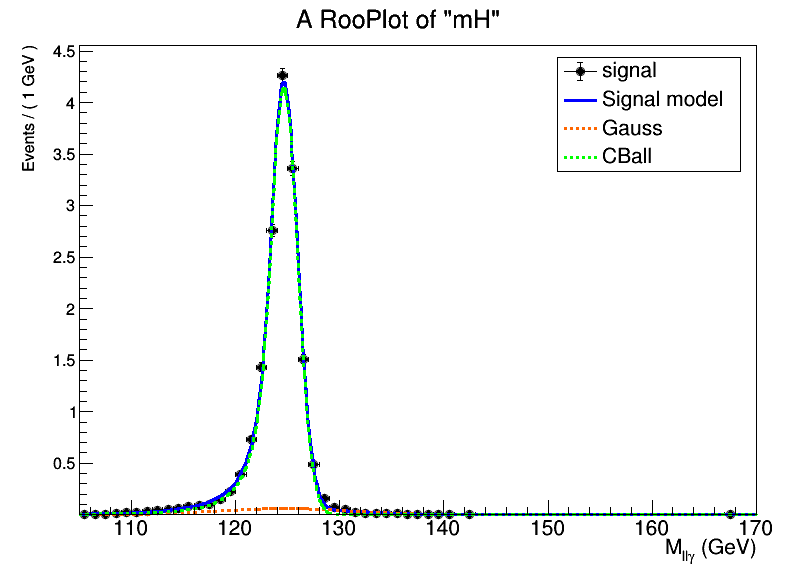
\includegraphics[width=0.40\textwidth]{fig/signal_fit/2018/sigfit_mu_ggF_3_125.png}
		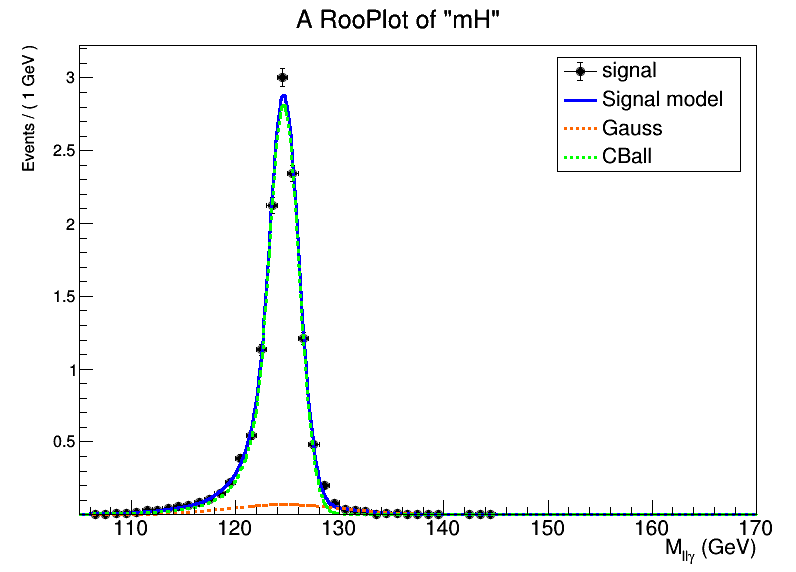
\includegraphics[width=0.40\textwidth]{fig/signal_fit/2018/sigfit_mu_ggF_4_125.png}\\
		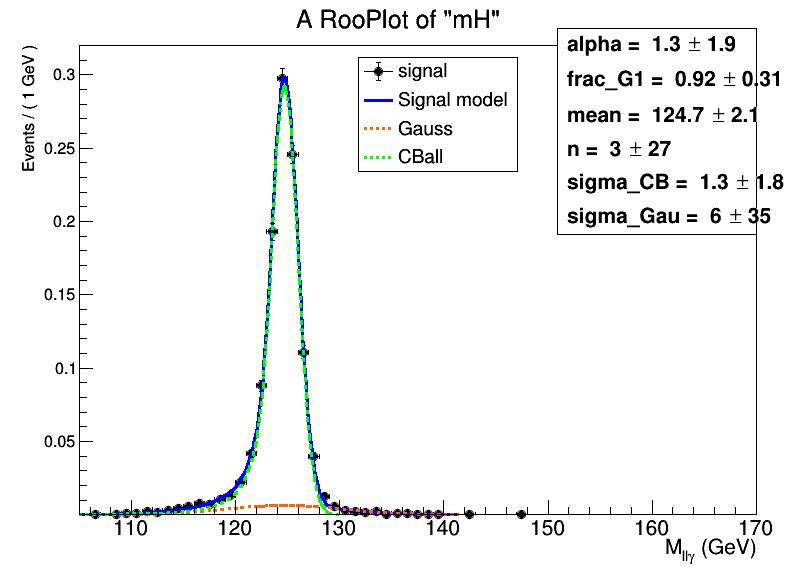
\includegraphics[width=0.40\textwidth]{fig/signal_fit/2018/sigfit_mu_VBF_501_125.png}
		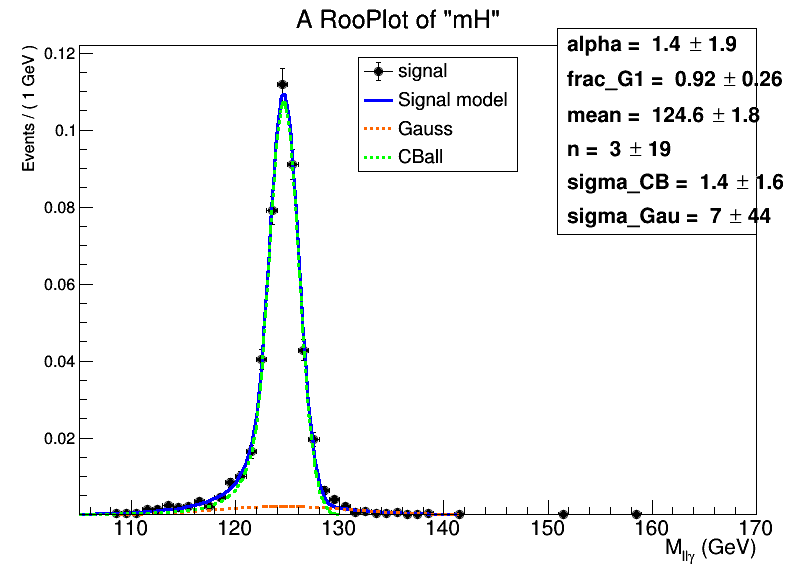
\includegraphics[width=0.40\textwidth]{fig/signal_fit/2018/sigfit_mu_VBF_502_125.png}\\
		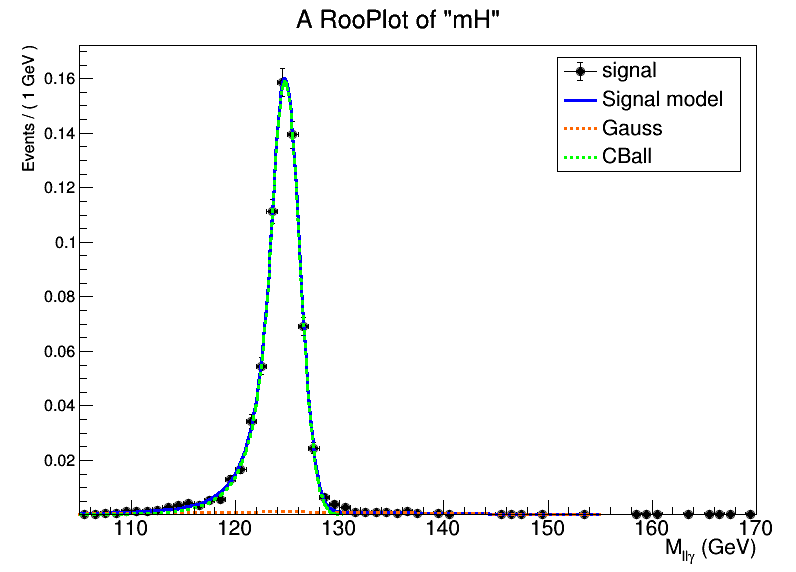
\includegraphics[width=0.40\textwidth]{fig/signal_fit/2018/sigfit_mu_VBF_503_125.png}\\
		\caption{Fits to simulated $m_{\ell^+\ell^-\gamma}$ signal distributions in the muon channel for
            		 $m_\PH=125\GeV$ for the 2018 data-taking period.
			 The blue line shows the total fit function, the green line shows the Crystal Ball function component, and the red line shows the Gaussian function component.
			 The top four plots correspond to the untagged categories, and the bottom three plots correspond to the dijet categories.}
		\label{fig:elesigfit}
	\end{center}
\end{figure}

\begin{figure}
	\begin{center}
	  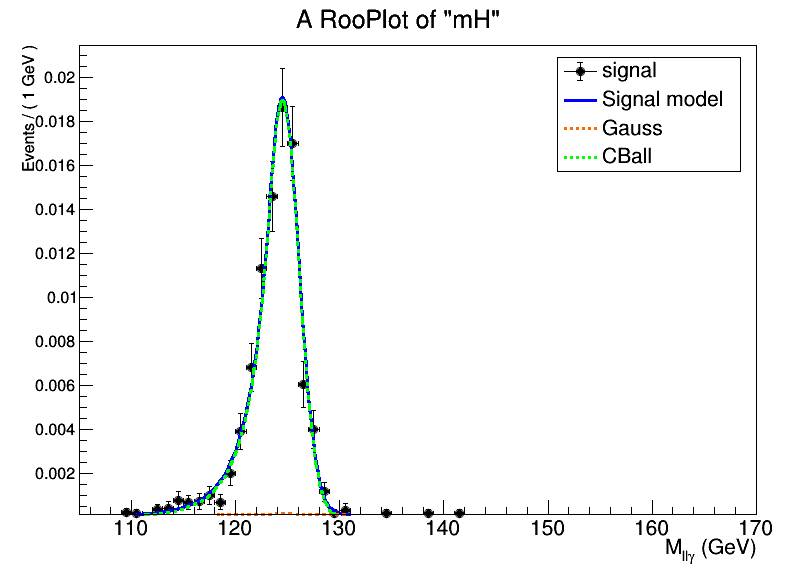
\includegraphics[width=0.40\textwidth]{fig/signal_fit/2018/sigfit_ele_mu_ZH_6789_125.png}
	  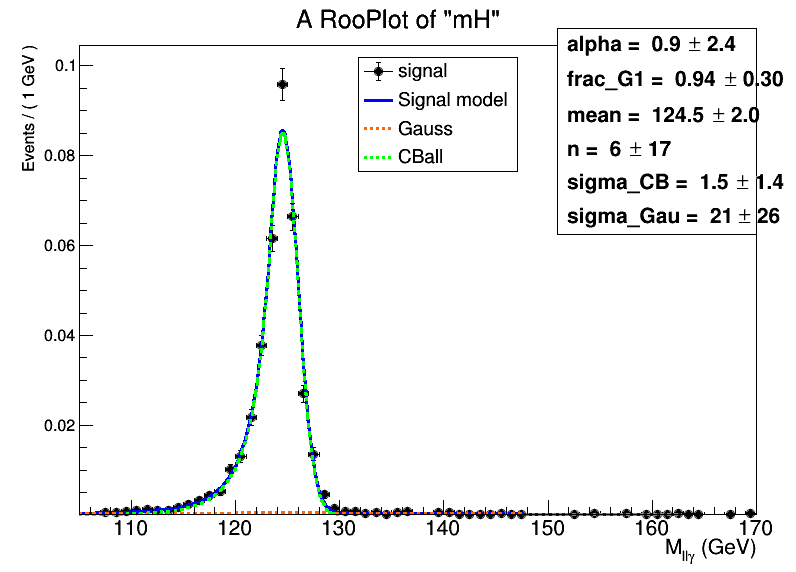
\includegraphics[width=0.40\textwidth]{fig/signal_fit/2018/sigfit_ele_mu_WH_6789_125.png}
		\caption{Fits to simulated $m_{\ell^+\ell^-\gamma}$ signal distributions in the electron and muon channels combined in the lepton-tagged category for
            		 $m_\PH=125\GeV$ for the 2018 data-taking period.
        		 The left plot shows the fit to simulated ZH production events, and the right plot shows the fit to simulated WH production events. 
			 The blue line shows the total fit function, the green line shows the Crystal Ball function component, and the red line shows the Gaussian function component.}
		\label{fig:elemusigfit}
	\end{center}
\end{figure}
